\documentclass{article}

\title {Network Address Translation}
\author{Antunez Joaquin, Gonzalez Alejo, Nielsen Maximiliano}
\date{Junio 2019}
 \usepackage{graphicx}
\begin{document}
 
\begin{titlepage}
\pagestyle{empty}
\maketitle
\thispagestyle{empty}
\end{titlepage}

\section*{Introducción Lab Nat con IPtables}

\subsection*{¿Qué es NAT?}

El proceso de Network Address Translation es un mecanismo usado por los routers IP para que dos redes puedan intercambiar paquetes aunque tengan direcciones incompatibles.
En una estructura donde varios hosts tienen direcciones IP privadas (red interna), cuando estos quieren enviar paquetes fuera del router NAT se encarga de traducir esa dirección interna (de rango privado) en una externa (de rango público).
Cuando se creo el Internet en el año 1969, no se lo pensó con la magnitud que hoy tiene.
El protocolo IPv4 consta 32 bits y, a día de hoy, un número limitado de direcciones IP; por eso es tan necesaria la NAT. Gracias a la misma se logra que, por ejemplo, en una red de una empresa donde hay cientos de computadoras, se arme una red interna donde cada host tiene una dirección interna (privada) y así se tenga solo una dirección pública o a lo sumo unas pocas más, en vez de tener cientos de direcciones públicas. Esto es fundamental para el ahorro de direcciones IP públicas IPv4 ya que estas, como todos sabemos, no son infinitas y en algún momento se van a agotar.\\
Los usuarios internos utilizan normalmente la Source NAT para acceder a Internet; la dirección de origen se traduce y por lo tanto se mantiene privada.
El NAT de destino se realiza en los paquetes entrantes cuando el firewall traduce una dirección de destino a una dirección de destino diferente; por ejemplo, traduce una dirección de destino pública a una dirección de destino privada.
\\
Para comenzar con el laboratorio primero crearemos la siguiente estructura:\\
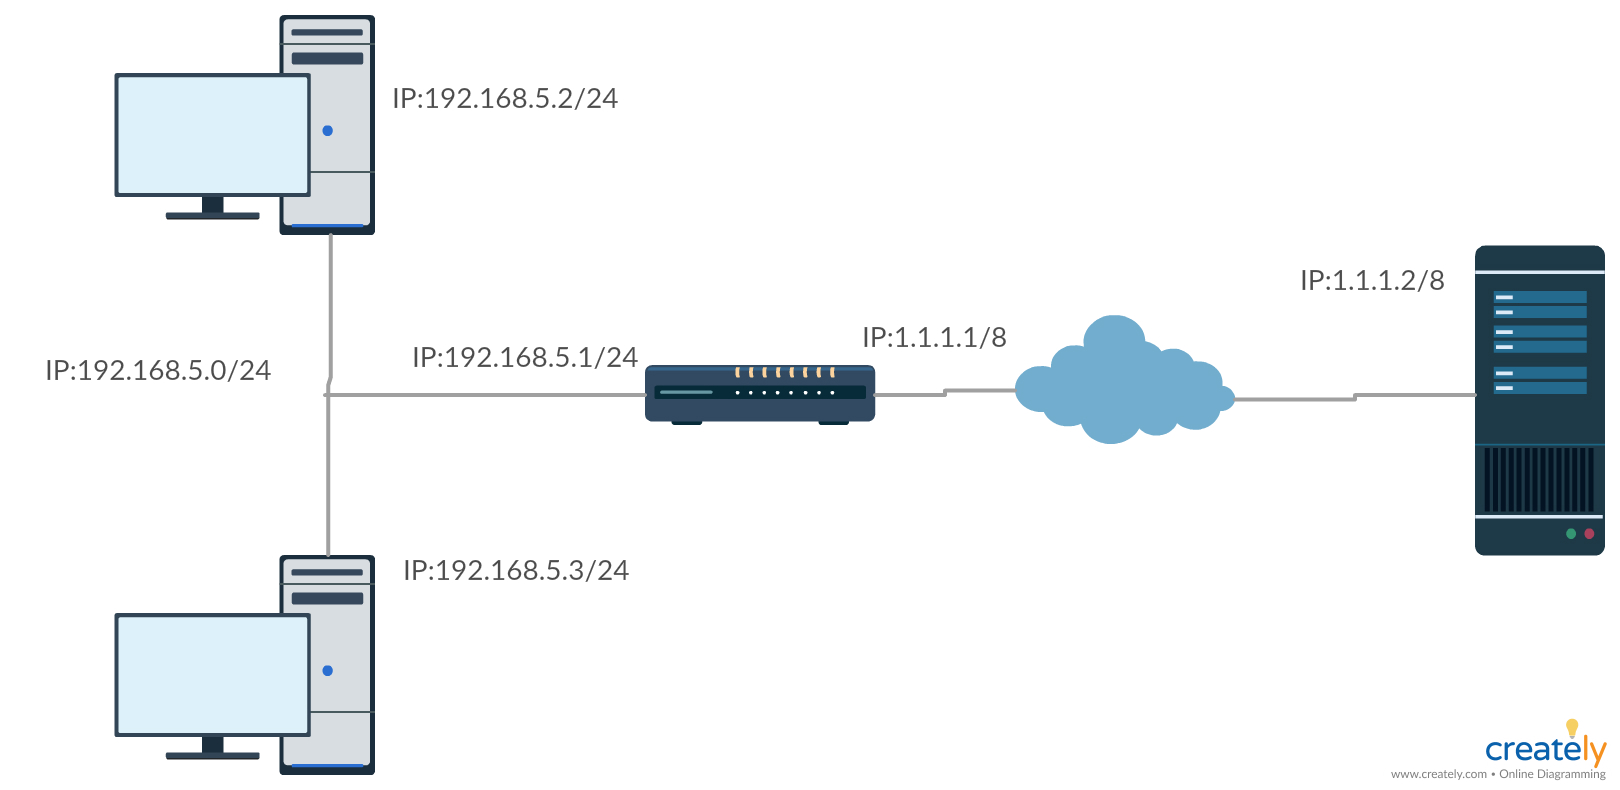
\includegraphics[width=\textwidth]{graficolab}
\\\\ \hfill \\
Como ven disponemos de una red interna con 2 hosts y una conexión a internet donde se encuentra un servidor con IP pública.\\
Quiere hacer Source NAT; cambiar la dirección de origen de las conexiones a algo diferente. Esto se hace en la cadena POSTROUTING, justo antes de que sea enviado. Este es un detalle importante, ya que significa que cualquier otro servicio de la máquina Linux (encaminamiento, filtrado de paquetes) verá el paquete sin cambiar.
El Source NAT se especifica indicando (-j SNAT), y la opción (--to) especifica una dirección IP, un rango de direcciones IP, y un puerto o rango de puertos opcionales (sólo con los protocolos UDP y TCP).\\
\hfill\\
\textit{iptables -t nat -A POSTROUTING -s 1.1.1.0/8 -j SNAT --to 192.168.5.1}
\\ \hfill \\
Este comando habilita que todo lo que tenga origen en la red 1.1.1.0/8 sera enviado a la interface del router del lado de la red privada.
\\ \hfill \\
Quiere hacer Destination NAT. Esto se hace en la cadena PREROUTING, según entra el paquete; esto significa que cualquier otro servicio de la máquina con Linux (encaminamiento, filtrado de paquetes) verá el paquete yendo a su destino (real) (el definitivo).
Destination NAT se especifica utilizando (-j DNAT), y la opción (--to) especifica una dirección IP, un rango de direcciones IP, y un puerto o rango de puertos opcionales (sólo para los protocolos UDP y TCP).\\\\ \hfill \\
\textit{iptables -t nat -A PREROUTING -d 1.1.1.0/8 -j DNAT --to 1.1.1.1}
\\\\ \hfill \\
Este comando habilita que todo paquete que tenga de destino la red 1.1.1.0/8 se envie a la interface de red del router que está del lado del servidor. 

\end{document}